\documentclass[letterpaper]{article}
\usepackage[bottom=.7in]{geometry}
\usepackage[utf8]{inputenc}
\usepackage[T1]{fontenc}
\usepackage[english]{babel}
\usepackage{fancyhdr}
\usepackage{graphicx}
\usepackage{caption}
\usepackage[breaklinks=true, hidelinks=true]{hyperref}
\usepackage[nottoc, numbib]{tocbibind}
\usepackage[
sorting=ynt
]{biblatex}
\addbibresource{bibliography.bib}

\pagestyle{fancy}
\pagenumbering{arabic}
\rhead{Angelica Urbanelli S271114}
\lhead{Data Spaces, a.y. 2020/2021}

\begin{document}
	\title{Tesina}
	\author{Angelica Urbanelli S271114}
	\date{Data Spaces, a.y. 2020/2021}
	\maketitle
	
	\tableofcontents
	
	\newpage 
	\section{Introduction}
	-spiegare il problema
		importanza di distinguere buoni e cattivi pagatori
		statistiche?
		
	-interpretabilità?
	-falsi buoni peggio di falsi cattivi
	
	
	\section{Dataset description}
	\subsection{History}
	The dataset used comes from the UCI Machine Learning Repository \cite{uci}, under the name "South German Credit (UPDATE) Data Set" \cite{dataset}. \\
	Ulrike Grömping, professor at the Beuth University in Berlin, in her paper \cite{gromping} provides the history of this dataset, her considerations about the data and corrections on the code table.\\
	Briefly, the data come from a large regional bank in the southern Germany that have been collected from 1973 to 1975, and have been originally provided to UCI in 1994 by Professor Dr. Hans Hofmann from Hamburg University \cite{hofmann} as part of a group of datasets in the context of the EU Statelog Project.\\
	Because of many inconsistencies, found while trying to interpret the final results of her experiments, Grömping decided to research the story of this data, that she found in the German literature together with the same dataset with some differences. These informations helped her	to fix the code table (a file that explains the encoding of categorical variables) of this dataset by providing a new one (now attached in the .zip downloadable from UCI).\\ 
	Grömping also explained that it was worth it because, although the dataset contains very old data, it is widely used in many researches in the domain of interpretable machine learning, indeed there are various R packages that include this data, and it \emph{is one of the few data sets on credit scoring that has a meaning attached to variables and their levels}, which is a very important feature when using this kind of data to do experiments whose interpretability is a key point of research.  \\
	
	\subsection{General structure}
	The dataset contains 1000 samples, each one characterized by 20 features and classified as \texttt{good} or \texttt{bad credit risk}, in particular there are 700 good ones and 300 bad ones [Figure \ref{fig:1}].  Customers with “good” credits perfectly complied with the conditions of the contract, while customers with “bad” credits did not comply with the contract as required.\\ As reported in the aforementioned paper \cite{gromping}, the actual percentage of bad credits was around 5\%, and examples of bad credit risk have been heavily oversampled. 
	
	\begin{center}
		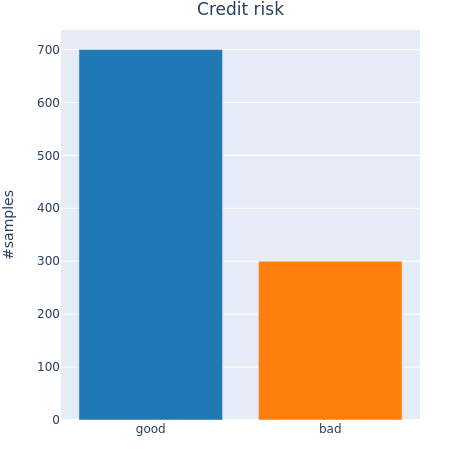
\includegraphics[scale=.35]{images/class.png}
		\captionof{figure}{caption}
		\label{fig:1}
	\end{center}
	
	\subsection{Features description}
	Among the 20 features, there are 3 numerical discrete variables:
	\begin{itemize}
		\item \textbf{duration}: credit duration in months
		\item \textbf{amount}: credit amount in DM\footnote{stands for Deutsche Mark, was the official currency of West Germany from 1948 until 1990 and later the unified Germany from 1990 until 2002 \cite{dm}}; it is the result of an unknown monotonic transformation, thus original values are not available
		\item \textbf{age}: age of the debtor in years
	\end{itemize}
	7 additional numerical variables that have been aggregated into a fixed number of intervals, so that they can be treated as ordinal ones:
	\begin{itemize}
		\item \textbf{employment\_duration}:  duration of debtor’s employment with current employer (unemployed; < 1 year ; $\geq$ 1 and < 4 years; $\geq$ 4 and < 7 years; $\geq$ 7 years)
		\item \textbf{installment\_rate}: : credit installments expressed as a percentage of debtor’s disposable income ( $\geq$ 35; $\geq$ 25 and < 35; $\geq$ 20 and < 25; < 20)
		\item \textbf{present\_residence}: from how many years the debtor lives in the present residence (< 1 year ; $\geq$ 1 and < 4 years; $\geq$ 4 and < 7 years; $\geq$ 7 years)
		\item \textbf{number\_credits}:  number of credits including the current one the debtor has (or had) at this bank (1; 2 or 3; 4 or 5; $\geq$ 6)
		\item \textbf{people\_liable}: number of people who financially depend on the debtor (i.e., are entitled to maintenance) (from 0 to 2; 3 or more)
		\item \textbf{status}: status of the debtor’s checking account with the bank in DM (no checking account; < 0; 0 $\leq$ ... < 200; $\geq$ 200 / salary for at least 1 year)
		\item \textbf{savings}: debtor’s savings in DM (unknown/no savings account; <  100; 100 $\leq$ ... <  500; 500 $\leq$ ... < 1000; $\leq$ 1000 )
	\end{itemize}
	10 categorical variables:
	\begin{itemize}
		\item \textbf{credit\_history}:  history of compliance with previous or concurrent credit contracts (delay in paying off in the past; critical account/other credits elsewhere; no credits taken/all credits paid back duly; existing credits paid back duly till now; all credits at this bank paid back duly )
		\item \textbf{purpose}:  purpose for which the credit is needed (others; car (new); car (used); furniture/equipment; radio/television; domestic appliances; repairs; education; vacation; retraining; business)
		\item \textbf{personal\_status\_sex}:  combined information on sex and marital status; sex cannot be recovered from the variable because male singles and female non-singles are coded with the same code; in addition, female widows are not listed in any of the categories (male divorced/separated; female non-single or male single; male married/widowed; female single)
		\item \textbf{other\_debtors}: whether there is another debtor or a guarantor for the credit (none; co-applicant; guarantor)
		\item \textbf{property}:  the debtor’s most valuable property, i.e. the highest possible code is used ( unknown / no property; car or other [savings don't fall into this category]; building society savings agreement (mortgage)/life insurance; real estate )
		\item \textbf{other\_installment\_plans}: installment plans from providers other than the credit-giving bank (bank; stores; none)
		\item \textbf{housing}:  type of housing the debtor lives in (for free; rent; own)
		\item \textbf{job}: quality of debtor’s job (unemployed/unskilled - non-resident; unskilled - resident; skilled employee/official; manager/self-employed/highly qualified employee)
		\item \textbf{telephone}:  whether there is a telephone landline registered on the debtor’s name; of course this variable would have no meaning nowadays, but this data come from 1970s (yes; no)
		\item \textbf{foreign\_worker}: whether the debtor is a foreign worker (yes; no)
	\end{itemize}	
	Among these categorical features, a further distinction can be done, by dividing ordinal and nominal ones. In the first group I considered the ones whose values can be ranked, that are \textbf{credit\_history}, \textbf{property} and \textbf{job}. 
	
	\section{Data preprocessing}
	\subsection{Labels encoding}
	All the features' labels are expressed as integers. Indeed, both nominal and ordinal values have been previously mapped to integers using label encoding from 0 to N-1 (only for \textbf{purpouse} and \textbf{credit\_history}) or from 1 to N (all the other variables) where N is the number of labels for a certain feature. Apparently there is no particular reason for which the donor of the data did this distinction. For what concerns class labels (\texttt{credit risk}), they have been mapped to $0$ for \texttt{bad} and $1$ for \texttt{good}. \\
	In order to make variables more uniform, two small changes have been done:
	\begin{itemize}
		\item the variable \textbf{installment\_rate} is the only one among the ordinal variables having a decreasing order, so its mapping has been inverted;
		\item \textbf{credit\_history}'s mapping has been changed from $0 \rightarrow 4$ to $1 \rightarrow 5$. Also \textbf{purpouse} has the same problem but it will be treated later.
	\end{itemize}
	In addition, all nominal variables have to be encoded in a different way with respect to the actual one ($1 \rightarrow N$). Indeed this encoding gives an arbitrary ranking to features that don't have one, and this is a problem when applying distance-based classification algorithms because those could potentially exploit this fictional structure created by the mapping itself. 
	\subsection{One hot encoding vs binary encoding}
	In order to perform this mapping I took into account two 
	\section{Missing values and outliers}
	\section{Dataset normalization}
	
	\section{Dataset Analysis}
	
	
	\section{preprocessing}
	-trovare outliers e decidere che farne
	
	-normalizzazione
	
	\section{Analysis}
	-distribuzione variabili
	-distribuzione variabili rispetto alle classi (scatter plot, violin plot)
	-correlazione variabili
	-t-SNE
	-clustering per vedere se mappa le label
	
	\section{dimensionality reduction}
	-eliminare/aggregare variabili correlate 
	-pca per capire quali sono le feature più importanti
		-lineare
		-kpca
	-eventualmente di nuovo correlazione tra variabili
	
	\section{prepare data for training}
	-oversampling
	-undersampling
	-smote
	-divisione training-test
	
	\section{classificazione}
	-logistic regression (also + regularization ridge or lasso)
	-tree
	-random forest (less simple to explain results)
	-svm (linear, rbf, polinomial, sigmoid)
	-knn
	-fda
	-qda?
	-lda? bayes?
	-eventually simple mlp
	
	\section{results}
	-per ogni combinazione (dim-reduction - algoritmo) fare ROC, accuracy, confusion matrix, recall, precision, F1 (armonic mean between precision and recall)
	-istogrammi ? 
	
	
	
	\newpage
	\printbibliography
	\addcontentsline{toc}{section}{References}
	
\end{document}